\documentclass[12pt, letterpaper, notitlepage, DIV=16, BCOR=1mm, headlines=2]{scrreprt}

\usepackage[hidelinks]{hyperref}
\usepackage[T1]{fontenc}
\usepackage{mathptmx}
\usepackage{graphicx}
\usepackage{siunitx}
%\graphicspath{{../}}

% make it a little easier on the eyes (next three line dark mode)
%\usepackage{xcolor}
%\pagecolor[rgb]{0,0,0} %black
%\color[rgb]{0.75,0.75,0.75} %grey

% make the default font times new roman
\setkomafont{disposition}{\rmfamily}

% make sure title and toc are on same page
\makeatletter
\newcommand*{\tocontents}{\@starttoc{toc}}
\makeatother

% add hyperlinks to toc
\hypersetup{
  linktoc=all
}

% adjust chapter height
\RedeclareSectionCommand[beforeskip=0pt]{chapter}

% remove page break before chapter titles
%\RedeclareSectionCommand[style=section]{chapter}

\title{AnalogIC Assignment 2}
\author{William Daniel Hiromoto}
\date{\today}

\begin{document}

\maketitle
%\tocontents{}

\chapter{Part A}
\section*{Question 1}
The W \& L values that satisfy the requirements was found by varying the minimum and maximum
allowable values of the transistor for each parameter and
choosing the parameters which maximized for output AC magnitude;
this process is shown in figures \ref{fig:L_para} - \ref{fig:W_para}.
It was found that $W = 16.3\mu m$ and $L = 0.18 \mu m$ provide an AC output magnitude
larger than 10V/V while keping the transistors in saturation as shown in figures
\ref{fig:ACmag1} -
\ref{fig:schematicA}.
In this instance, the $V_{ds}$ is limiting the voltage swing as the output voltage
is closer in value to $V_{th}$ than $V_{DD}$; the output swing is $217.198mV$.

% W/L values with AC gain larger than 10V/V
\begin{figure}[h]
	\makebox[\textwidth]{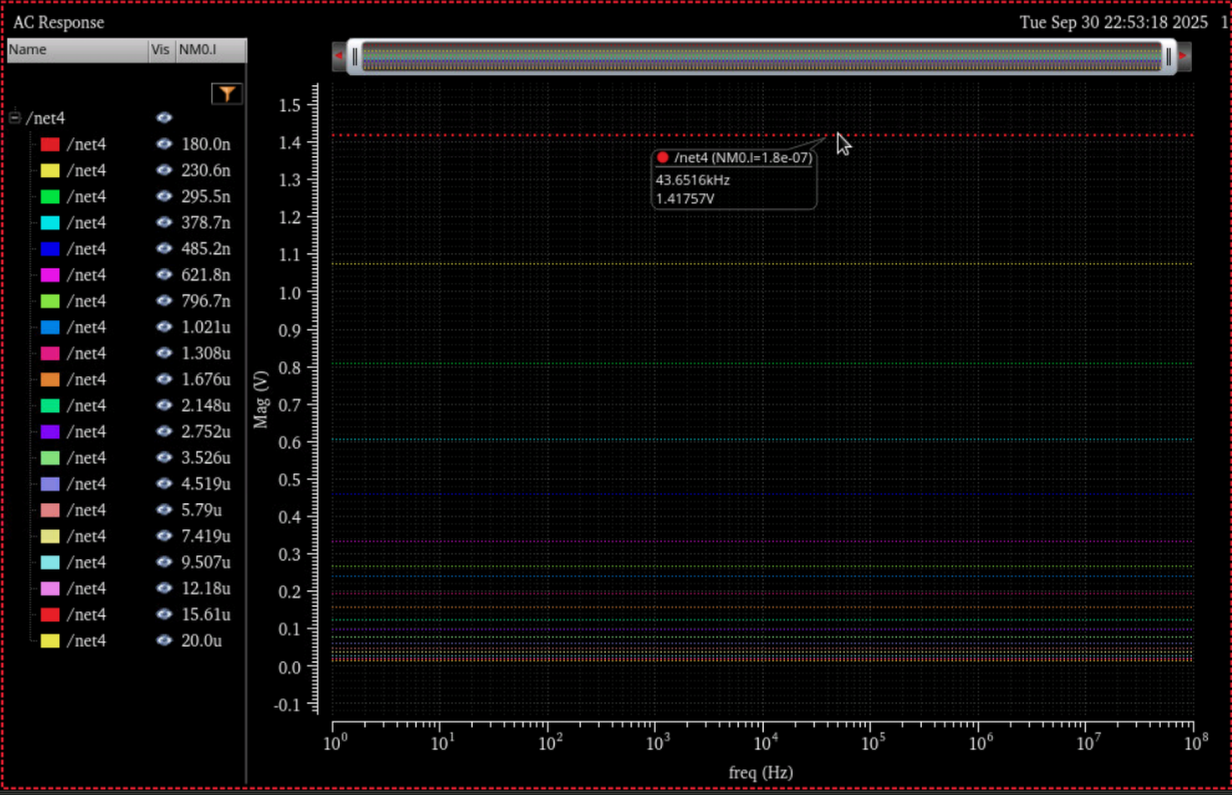
\includegraphics[width=\textwidth]{../partAImages/L_parametric.png}}
	\caption{AC magnitude results with $W=1\mu m$ and Length varied}
	\label{fig:L_para}
\end{figure}

\begin{figure}[h]
	\makebox[\textwidth]{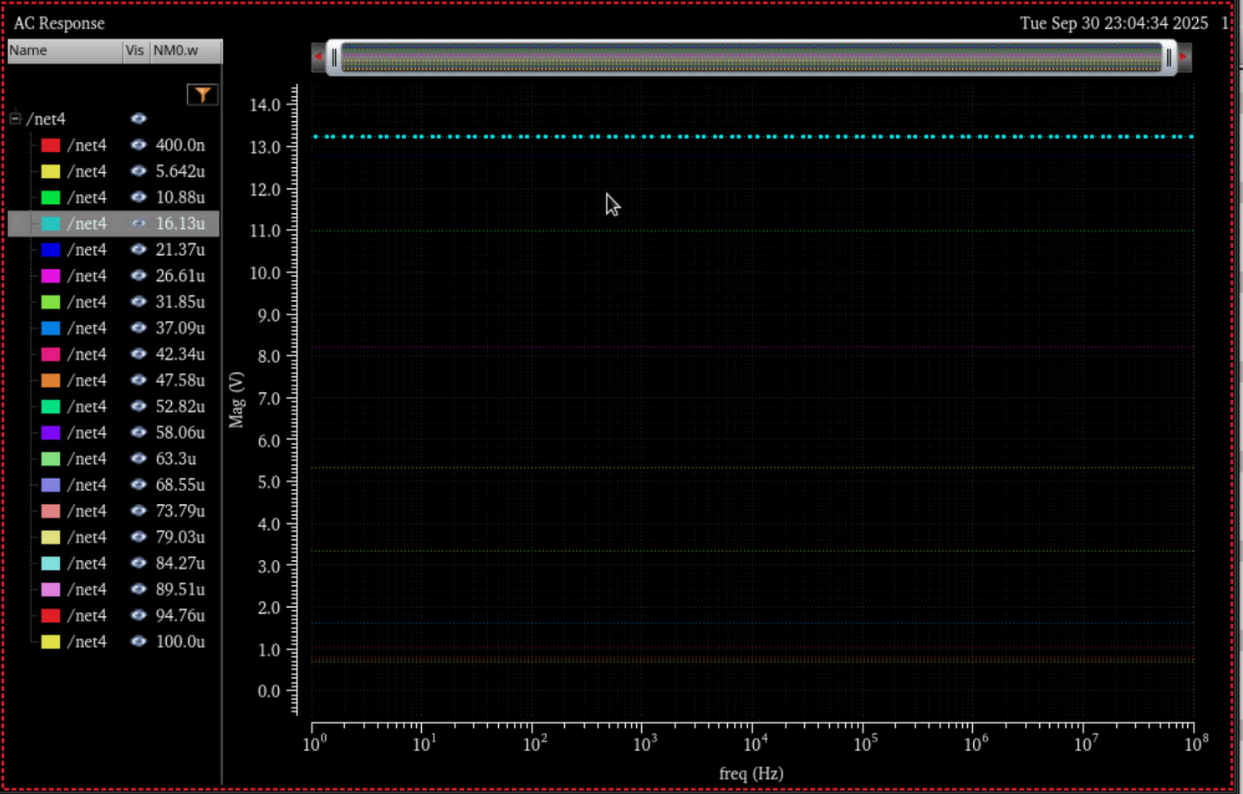
\includegraphics[width=\textwidth]{../partAImages/W_parametric.png}}
	\caption{AC magnitude results with $L=0.18\mu m$ and Width varied}
	\label{fig:W_para}
\end{figure}

% graph of AC magnitude result
\begin{figure}[h]
	\makebox[\textwidth]{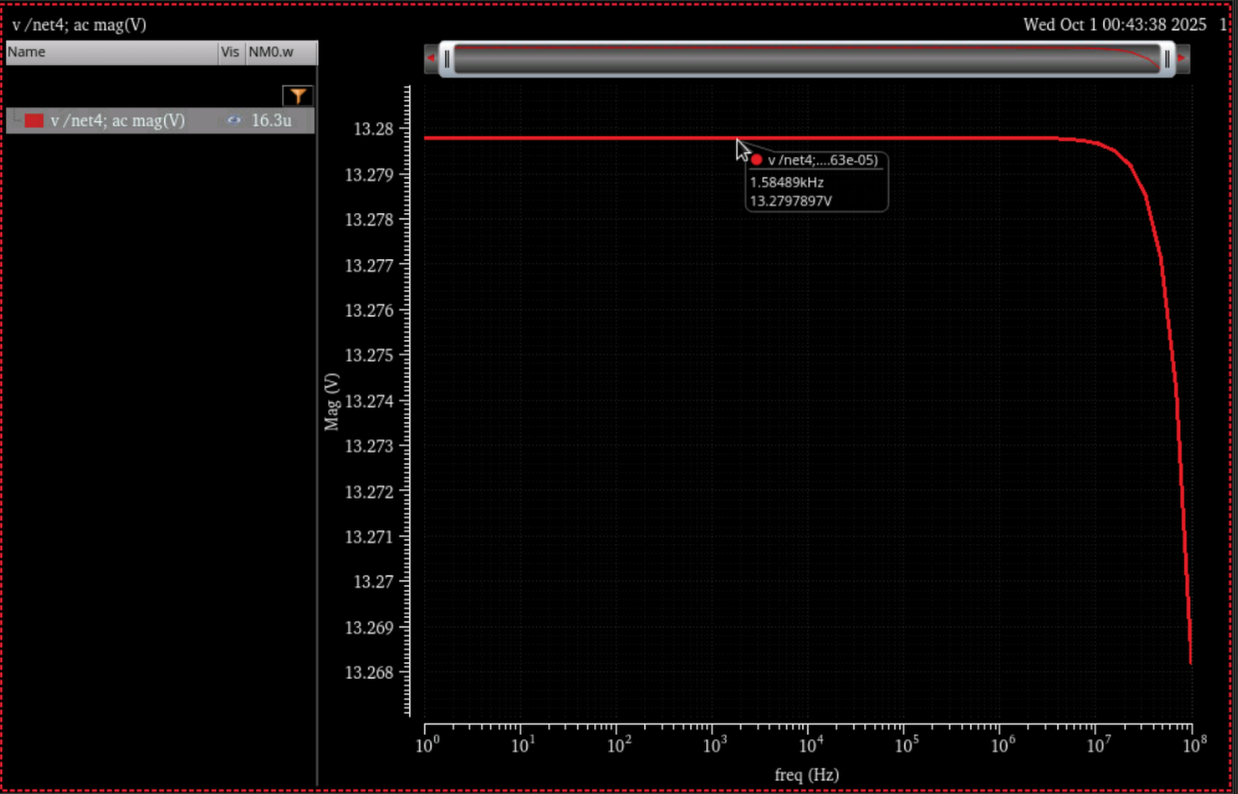
\includegraphics[width=\textwidth]{../partAImages/parameters.png}}
	\caption{AC magnitude results with $W=16.13\mu m$ and $L=0.18\mu m$}
	\label{fig:ACmag1}
\end{figure}
% schematic with DC operating point annotations
\begin{figure}[h]
	\makebox[\textwidth]{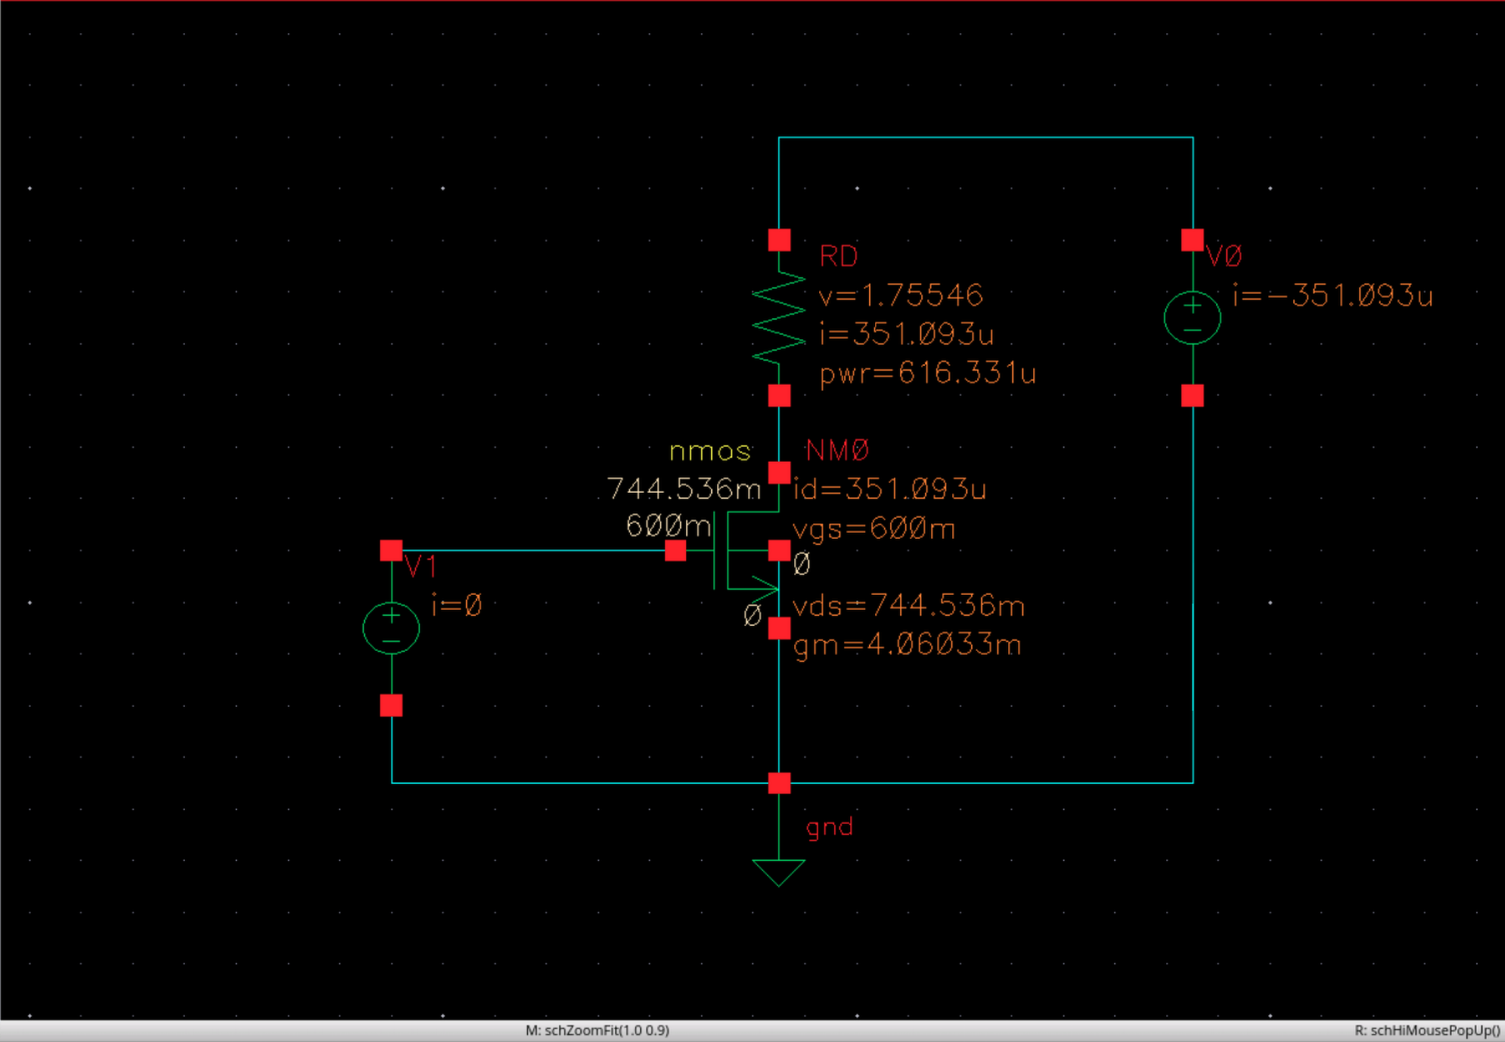
\includegraphics[width=\textwidth]{../partAImages/Schematic.png}}
	\caption{Schematic of circuit with DC operating points shown for $W=16.13\mu m$ and $L=0.18\mu m$}
	\label{fig:schematicA}
\end{figure}

% does Vds or VDD limit the swing?
% to find output swing, and take veff with vout and vdd to find the max output swing/range
\section*{Question 2}
\begin{figure}[h]
	\makebox[\textwidth]{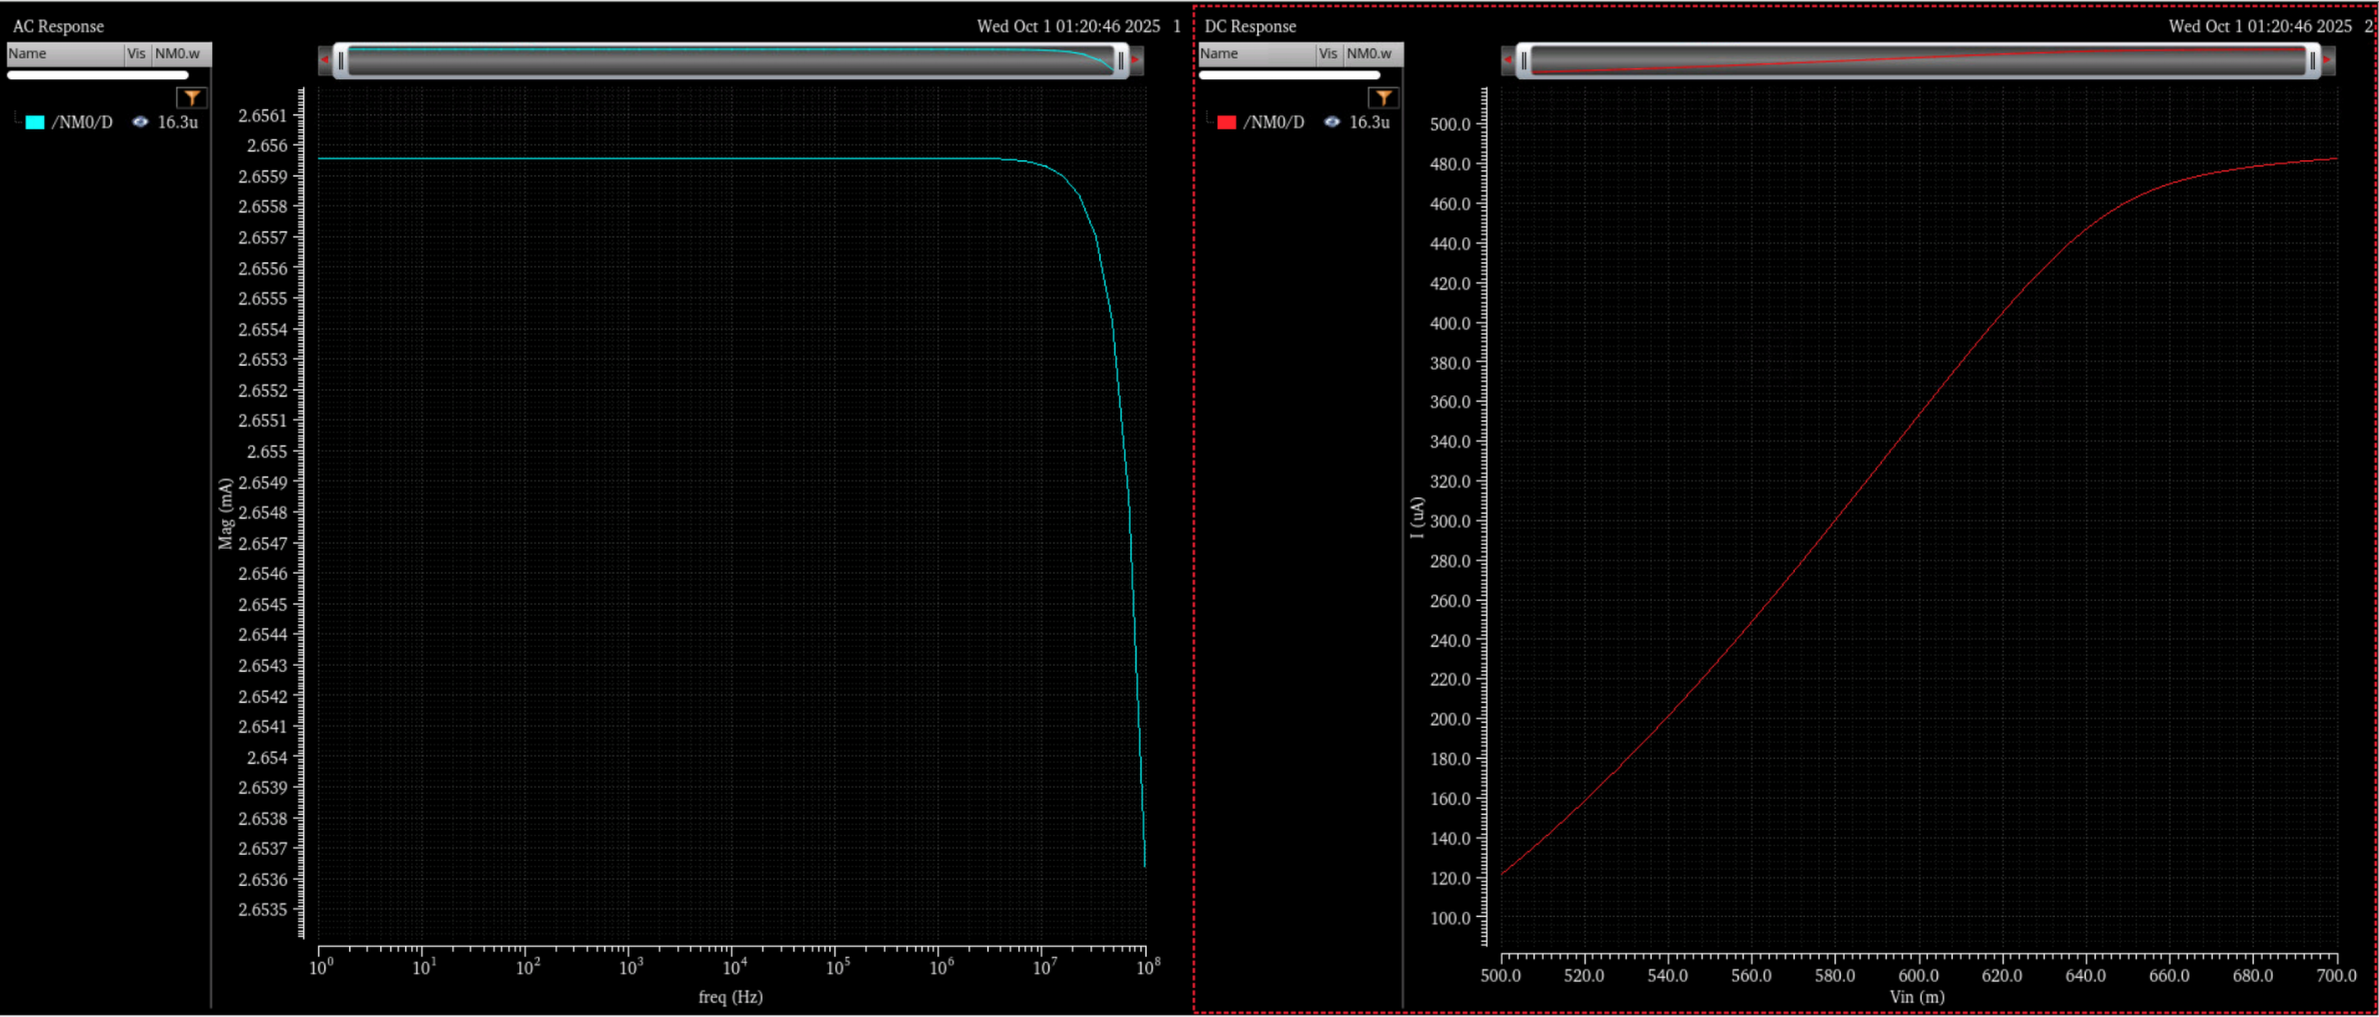
\includegraphics[width=\textwidth]{../partAImages/DCvary.png}}
	\caption{output DC current with $\pm 10mV$}
	\label{fig:DCVary}
\end{figure}



\chapter{Part B}
\section*{Question 1}
The same process as Part A Question 1 was used to find the W \& L Values
(figures \ref{fig:L_para2}
 - \ref{fig:W_para2}), 
being $W = 42.34\mu m$ and $L = 0.18 \mu m$. The results can be shown in
figures \ref{fig:ACmag2}
and \ref{fig:schematicB}.
The DC current of this amplifier was $351.093\mu A$.
The output swing found is $229.907mV$, which is limited by $V_{ds}$.

% W/L values with AC gain larger than 2.5V/V
\begin{figure}[h]
	\makebox[\textwidth]{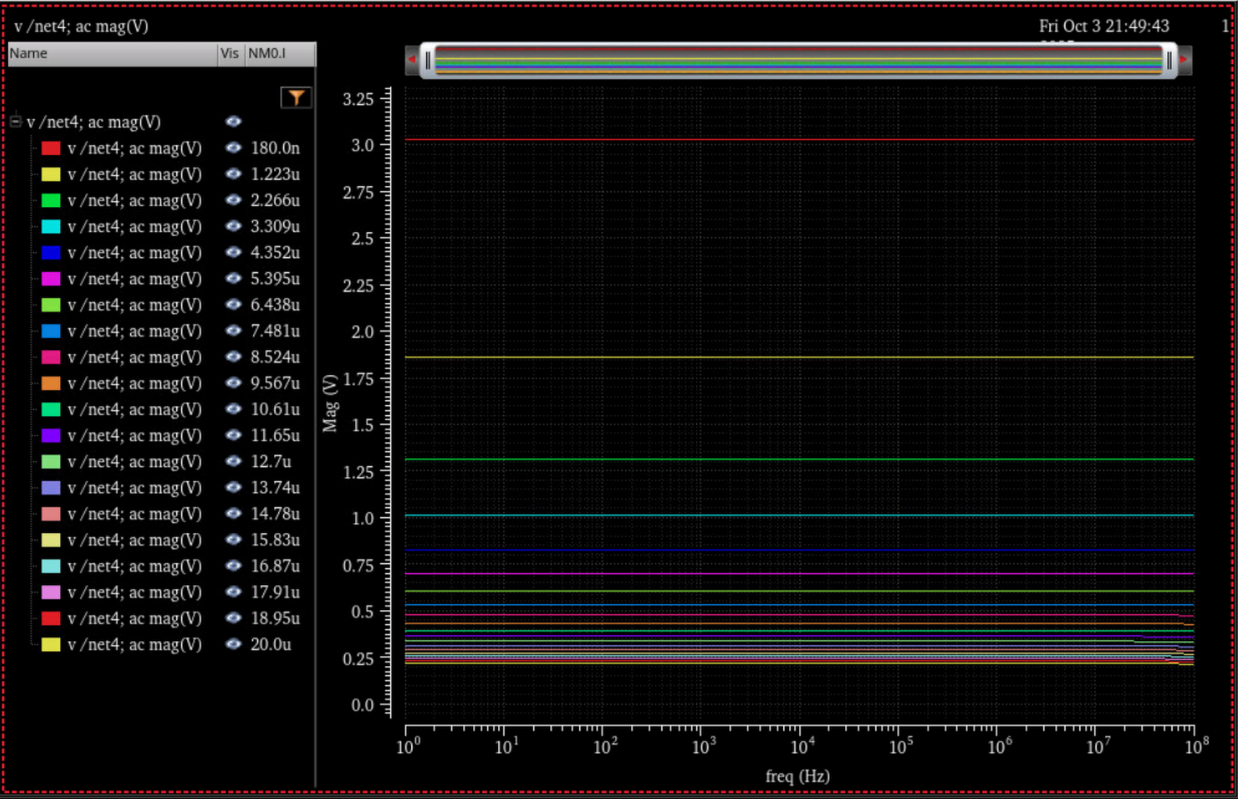
\includegraphics[width=\textwidth]{../partBImages/L_parametric.png}}
	\caption{AC magnitude results with $W=3\mu m$ and Length varied}
	\label{fig:L_para2}
\end{figure}

\begin{figure}[h]
	\makebox[\textwidth]{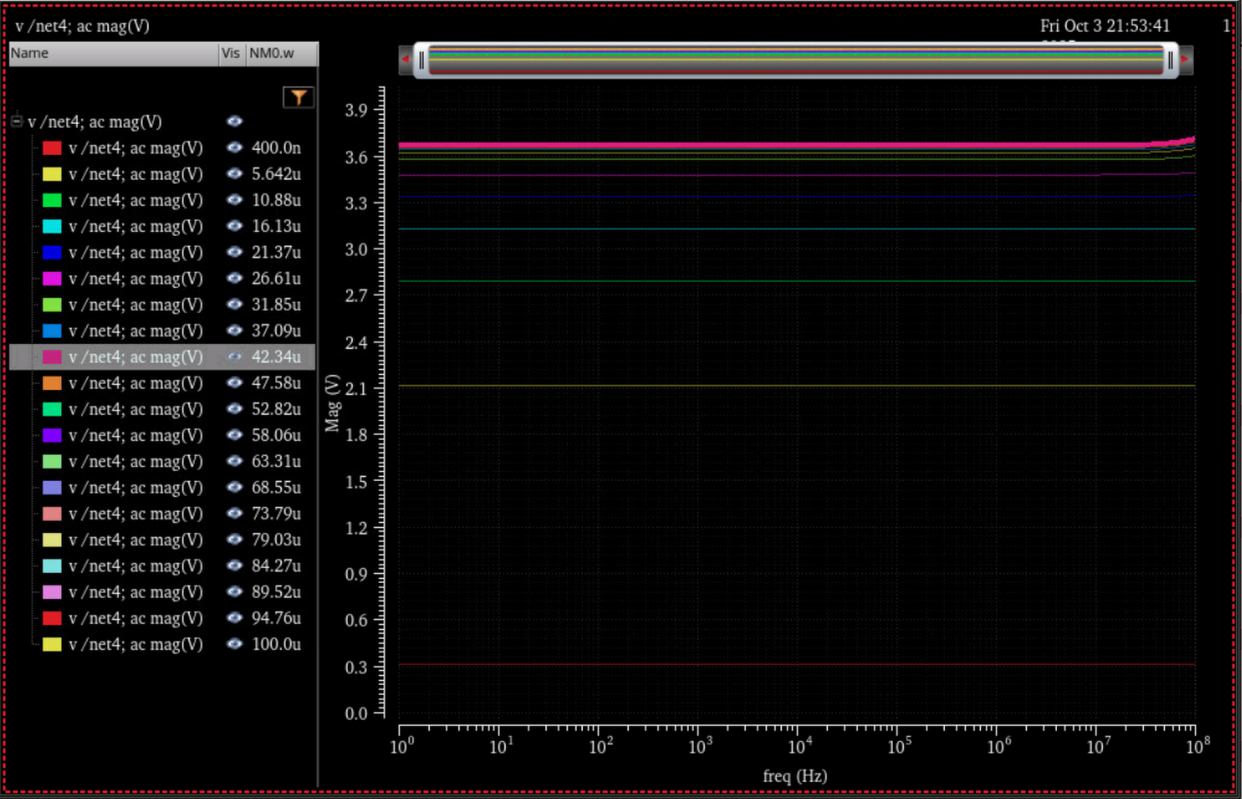
\includegraphics[width=\textwidth]{../partBImages/W_parametric.png}}
	\caption{AC magnitude results with $L=0.18\mu m$ and Width varied}
	\label{fig:W_para2}
\end{figure}

% graph of AC magnitude result
\begin{figure}[h]
	\makebox[\textwidth]{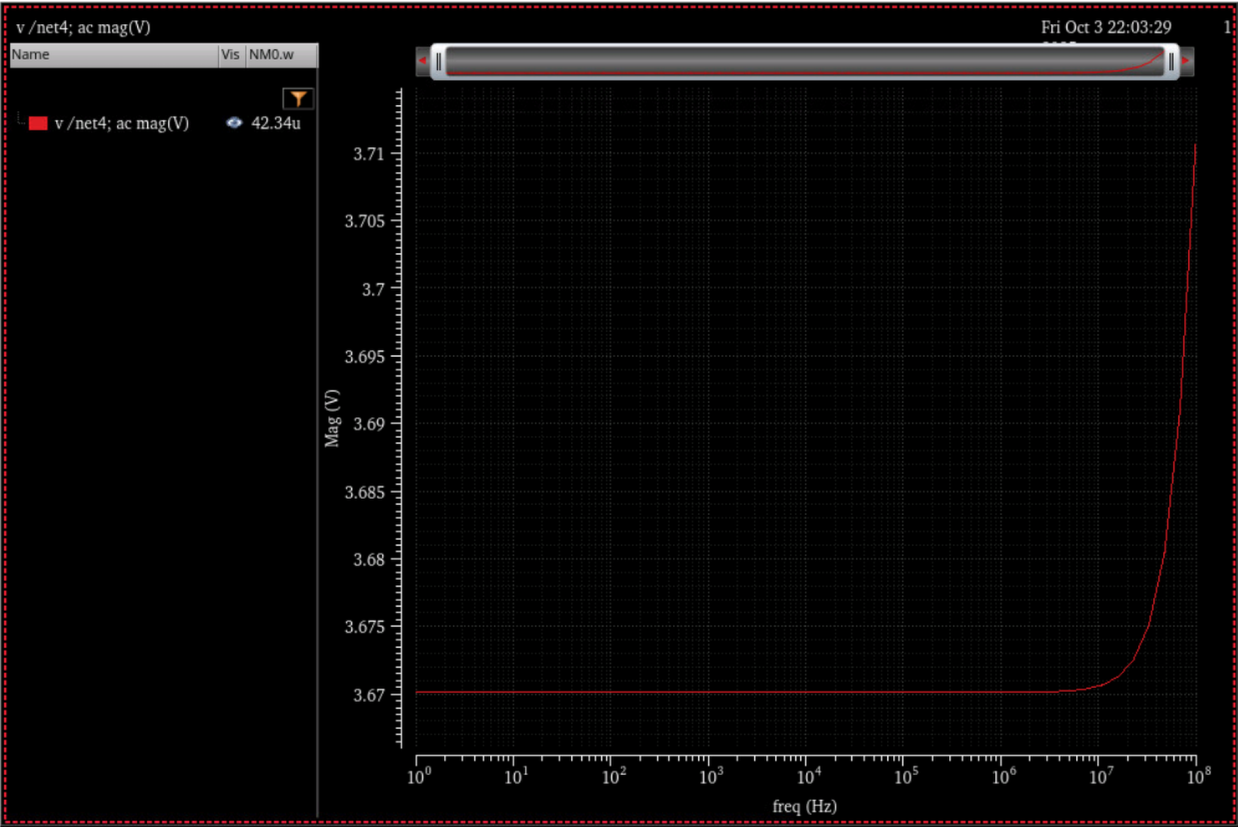
\includegraphics[width=\textwidth]{../partBImages/parameters.png}}
	\caption{AC magnitude results with $W=42.34\mu m$ and $L=0.18\mu m$}
	\label{fig:ACmag2}
\end{figure}
% schematic with DC operating point annotations
\begin{figure}[h]
	\makebox[\textwidth]{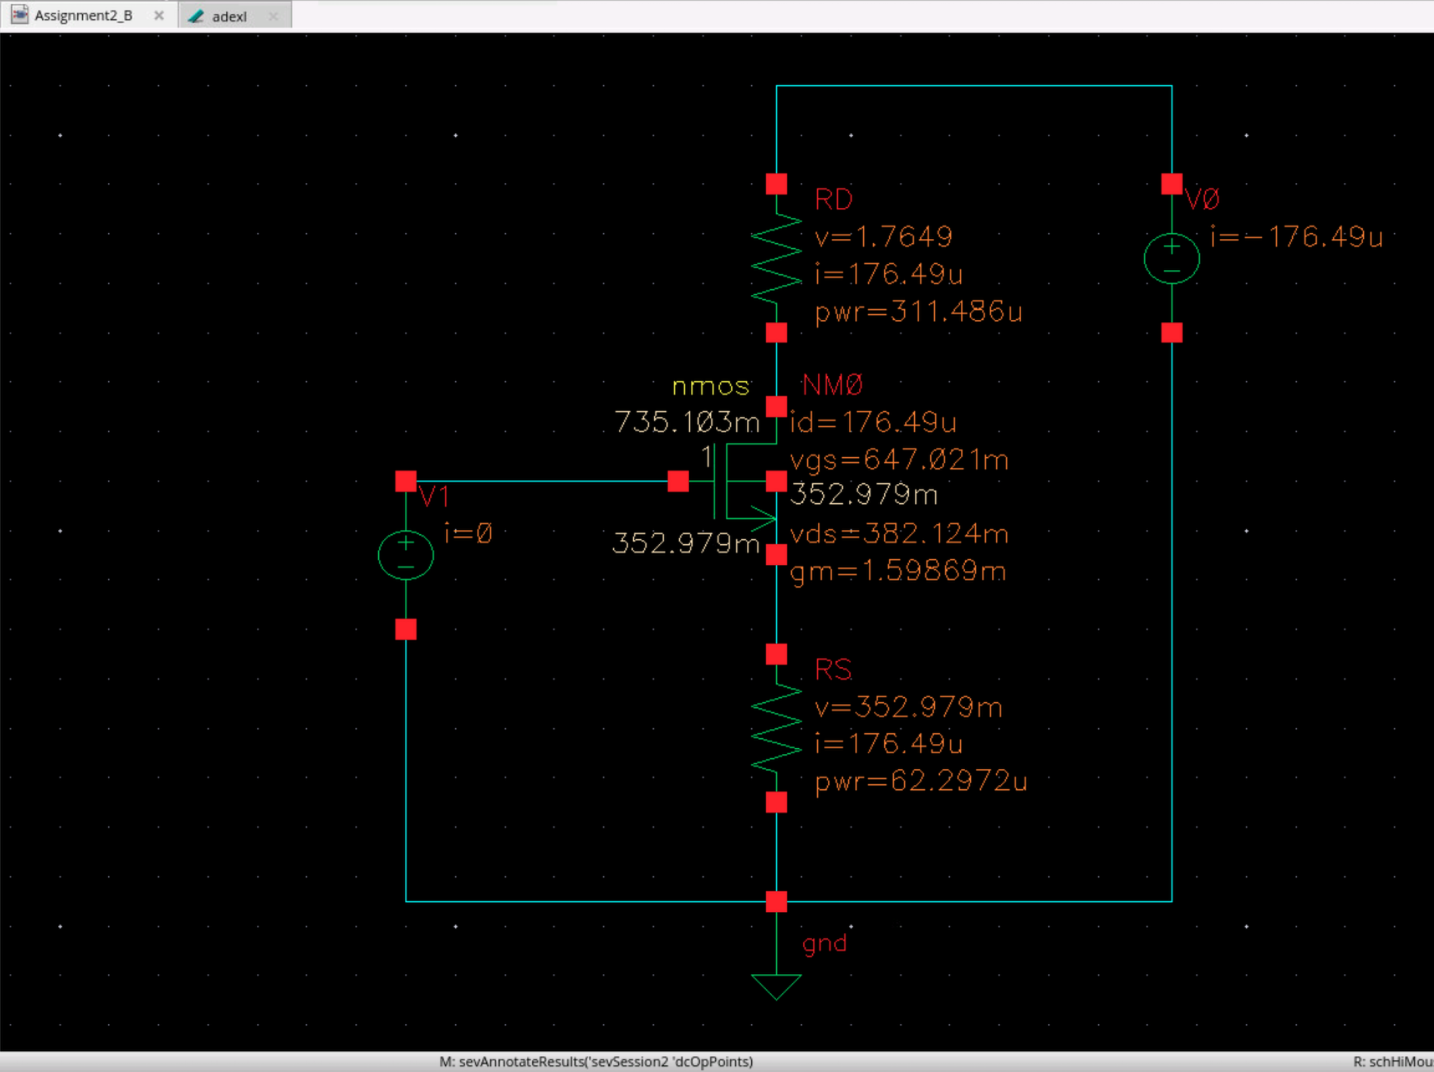
\includegraphics[width=\textwidth]{../partBImages/Schematic.png}}
	\caption{Schematic of circuit with DC operating points shown for $W=42.34\mu m$ and $L=0.18\mu m$}
	\label{fig:schematicB}
\end{figure}
% DC current of amplifier
% output swing of amplifier
% what limits the swing

\section*{Question 2}

\begin{figure}[h]
	\makebox[\textwidth]{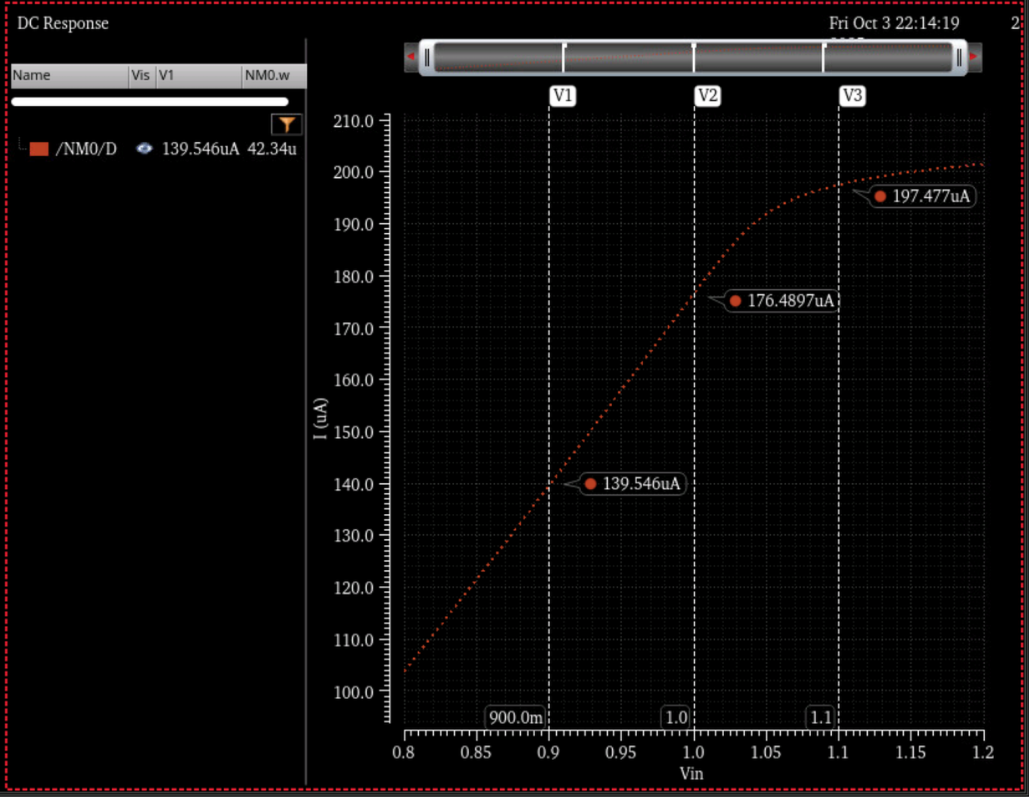
\includegraphics[width=\textwidth]{../partBImages/DCvary.png}}
	\caption{output DC current with $\pm 10mV$}
	\label{fig:DCVary2}
\end{figure}

\end{document}